\lhead[\thepage]{CAPÍTULO \thechapter. INTERFAZ DE PATRONES DE PROG\acrshort{ram}ACIÓN PARALELA PARA MEMORIA DISTRIBUIDA}
\chead[]{}
\rhead[Patrones de programación paralelos de alto nivel en arquitecturas de memoria distribuida\leftmark]{\thepage}
\renewcommand{\headrulewidth}{0.5pt}

\lfoot[]{}
\cfoot[]{}
\rfoot[]{}
\renewcommand{\footrulewidth}{0pt}

%% This is an example first chapter.  You should put chapter/appendix that you
%% write into a separate file, and add a line \include{yourfilename} to
%% main.tex, where `yourfilename.tex' is the name of the chapter/appendix file.
%% You can process specific files by typing their names in at the 
%% \files=
%% prompt when you run the file main.tex through LaTeX.
\chapter{Interfaz de patrones de programación paralela para memoria distribuida}
\label{ch:interfaz_patrones_memoria_distribuida}
\markboth{}{INTERFAZ DE PATRONES DE PROG\acrshort{ram}ACIÓN PARALELA PARA MEMORIA DISTRIBUIDA}

Este capítulo presenta la implementación realizada de \acrshort{grppi} para plataformas de memoria distribuida. En primer lugar se describe el problema (Sección \ref{sec:descripcion_problema}) por el cual se decide realizar esta implementación. Posteriormente, se describe la política de ejecución \acrshort{mpi} para \acrshort{grppi} (Sección \ref{sec:politica_ejecucion_mpi}), describiendo la interfaz de usuario resultante (Sección \ref{sec:interfaz_usuario}), la implementación de las colas de comunicación entre procesos (Sección \ref{sec:colas_comunicacion}) y el algoritmo de distribución de operadores en procesos \acrshort{mpi} (Sección \ref{sec:algoritmo_distribucion_mpi}).

\section{Descripción del problema}
\label{sec:descripcion_problema}

En general, la implementación de un back-end distribuido mediante \acrshort{mpi} se ha motivado principalmente por las necesidades de escalamiento y el desarrollo de nuevos modelos de programación para aplicaciones científicas \acrshort{dasp}. El interés de implementar este back-end proviene de la amplia adopción de \acrshort{mpi} en las supercomputadoras de hoy, que actualmente no tiene soporte estándar para el procesamiento de streaming~\cite{peng2017}. Debido a este motivo al crecimiento en los últimos años del paradigma del \emph{Big Data}, creemos necesario presentar un back-end que pueda ser de ayuda en el desarrollo de aplicaciones de streaming en C ++.

Por otro lado, una vez analizado el estado de la cuestión y las herramientas y frameworks actualmente disponibles para este área, identificamos una brecha importante entre la comunidad de \acrshort{mpi} y las necesidades de procesamiento de flujo de las aplicaciones científicas actuales ~\cite{stream2016}. En este sentido, el objetivo del nuevo back-end de \acrshort{grppi} \acrshort{mpi} es doble. Por un lado, \acrshort{grppi} ofrece una interfaz C ++ de alto nivel de patrones paralelos que mejora tanto la flexibilidad de la aplicación como la legibilidad del código fuente. Por otro lado, el uso de \acrshort{grppi} \acrshort{mpi} permite de forma transparente la ejecución de la aplicación de C ++ en tiempo real en plataformas \acrshort{hpc} distribuidas, ya que \acrshort{grppi} oculta la complejidad relacionada con la comunicación y la sincronización de procesos.

\section{Política de ejecución \acrshort{mpi} para \acrshort{grppi}}
\label{sec:politica_ejecucion_mpi}

Con respecto a la interfaz de patrones paralelos, hemos aprovechado \acrshort{grppi}, una interfaz de patrones paralelos genérica y reutilizable para aplicaciones C ++. Esta interfaz aprovecha al máximo las características modernas de C ++, los conceptos de metaprogramación y la programación genérica para actuar como un interruptor entre , hilos de C ++ y los modelos de programación paralela de Intel \acrshort{tbb}.  Su diseño permite a los usuarios aprovechar los marcos de ejecución antes mencionados en una interfaz única y compacta, ocultando la complejidad detrás del uso de mecanismos de concurrencia. Además, la modularidad de \acrshort{grppi} permite integrar fácilmente nuevos patrones, combinándolos para organizar construcciones más complejas. Además, permite la integración de nuevas políticas de ejecución basadas en modelos de programación distribuidos y de memoria compartida. Gracias a estas propiedades, \acrshort{grppi} se puede utilizar para implementar una amplia gama de aplicaciones existentes de procesamiento de datos y de streaming con esfuerzos relativamente pequeños, teniendo como resultado códigos portátiles que se pueden ejecutar en múltiples plataformas.

Como se indicó anteriormente, el objetivo de \acrshort{grppi} es acomodar una capa de patrones paralelos entre desarrolladores y marcos de programación paralelos existentes. Hasta ahora, \acrshort{grppi} solo admite políticas de ejecución de memoria compartida, como C + + Threads, e Intel \acrshort{tbb}. Para extender \acrshort{grppi} a fin de admitir plataformas distribuidas, hemos incorporado la política de ejecución de \acrshort{mpi} que, en este momento, permite a los usuarios ejecutar los patrones de oleoductos y flujos de granja en clusters de múltiples núcleos. En esta sección, describimos en detalle los elementos básicos de la política de ejecución de \acrshort{mpi}: \emph{i)} interfaz de usuario; \emph{ii)} canales de comunicación interna; y \emph{iii)} algoritmo de distribución de operadores.

\subsection{Interfaz de usuario}
\label{sec:interfaz_usuario}

Dado el diseño \acrshort{grppi}, donde cada política de ejecución se implementa utilizando una clase C ++, para la nueva política \acrshort{mpi} también diseñamos su clase. Esto se debe a que cada una de estas clases contiene las implementaciones de patrones específicos del marco junto con los parámetros de configuración para esa política. Básicamente, las interfaces de patrones \acrshort{grppi} están sobrecargadas con una implementación diferente para cada una de las políticas de ejecución disponibles. Con él, cuando se compila el código de usuario, la implementación del patrón específico se selecciona dependiendo de la política de ejecución pasada como argumento (ver parámetro \texttt{execution\_policy} en la interfaz del patrón Pipeline en la Figura \ref{fig:grppi-Pipeline-pattern}). El Listado~\ref{lst:parallel-exec-mpi} muestra un extracto de la clase de política de ejecución de \acrshort{mpi}. Tenga en cuenta que hemos utilizado la biblioteca Boost \acrshort{mpi} \cite{boost-mpi} como interfaz de C ++ \acrshort{mpi}. 

Como se observa, los constructores de políticas de ejecución reciben los argumentos del programa o el comunicador \acrshort{mpi} directamente. Para admitir escenarios híbridos, ambos constructores pueden recibir una política de ejecución de memoria compartida local. Esta política local se usará para ejecutar múltiples etapas de Pipeline o réplicas de Farm (también denominadas operadores de flujo) dentro del mismo proceso. Por lo tanto, los operadores asignados al mismo proceso se ejecutarán en forma secuencial o en paralelo según la política de ejecución de la memoria compartida seleccionada. 

\vspace{0.35cm}
%\vspace{-0.2cm}
\begin{lstlisting}[linewidth=1\columnwidth,caption={Clase de política de ejecución \acrshort{mpi} en \acrshort{grppi}.},label=lst:parallel-exec-mpi,frame=single]
template<typename LocalPolicy = parallel_execution_native>
class parallel_execution_mpi {
 namespace mpi = boost::mpi;
 ...
 public:
  parallel_execution_mpi(int argc, char** argv, 
          LocalPolicy local_exec_policy = parallel_execution_native{});
  parallel_execution_mpi(mpi::communicator mpi_comm = mpi::communicator{}, LocalPolicy local_exec_policy = parallel_execution_native{});
  ...                           
};
\end{lstlisting}
\vspace{0.35cm}

Como se muestra en el Listado~\ref{lst:Pipeline-example}, el patrón de Pipeline \acrshort{grppi} aprovecha la nueva clase de política de ejecución \acrshort{mpi} para su ejecución. Tenga en cuenta que la política se construye en la declaración utilizando los argumentos \texttt{argc} y \texttt{argv}. Esta canalización consta de tres etapas en la forma \texttt{(p|f|p)}, donde la primera y la tercera etapa se ejecutan en serie, mientras que la segunda ejecuta dos réplicas del mismo operador utilizando el patrón de la granja. Suponiendo que el programa se ejecute mediante 4 procesos de \acrshort{mpi}, el primero y el último respectivamente ejecutan las etapas de generador y consumidor, mientras que el segundo y el tercero calcularán cada una de las réplicas de conjunto. Es importante destacar que los artículos que transitan de una etapa a otra se envían y reciben a través de las colas de comunicación \acrshort{mpi} implementadas dentro de la política de respaldo.

\vspace{0.35cm}
\begin{lstlisting}[linewidth=1\columnwidth,caption={Ejemplo de Pipeline \acrshort{grppi} distribuido.},label={lst:Pipeline-example},frame=single]
grppi::parallel_execution_mpi ex{argc, argv};
grppi::Pipeline(ex, 
  [x=1,n]() mutable -> optional<double> { 
    if (x<=n) return x++;
    else return {}; 
  },
  grppi::Farm(2,[](double x) {
    return x*x;
  }),
  [](double x) { cout << x << endl; }
);
\end{lstlisting}
\vspace{0.35cm}

Los Listados~\ref{fig:grppi-Pipeline-pattern}, ~\ref{fig:grppi-Farm-pattern} muestra los prototipos C ++ \acrshort{grppi} \acrshort{mpi} de los patrones Pipeline y Farm. Tenga en cuenta el uso de \texttt{templates} con parámetros únicos y múltiples (pack) como referencias universales, lo que permite pasar múltiples objetos invocables (por ejemplo, un functor o expresión lambda) como para los operadores de patrones. Tenga en cuenta también que el primer parámetro indica la política de ejecución que se utilizará para ejecutar los operadores.

\vspace{0.35cm}
\begin{lstlisting}[linewidth=1\columnwidth,caption={Interfaz patrón Pipeline en \acrshort{grppi} \acrshort{mpi}.},label={fig:grppi-Pipeline-pattern},frame=single]
template <typename E, typename G, typename ... O>
void Pipeline(E execution_policy, G && generator, O && ... operators);
\end{lstlisting}
\vspace{0.35cm}

\begin{lstlisting}[linewidth=1\columnwidth,caption={Interfaz patrón Farm en \acrshort{grppi} \acrshort{mpi}.},label={fig:grppi-Farm-pattern},frame=single]
template <typename O>
void Farm(int replicas_replicas, O && operators);  
\end{lstlisting}
\vspace{0.35cm}

\subsection{Colas de comunicación}
\label{sec:colas_comunicacion}

Los canales de comunicación son fundamentales en las aplicaciones de \acrshort{dasp} distribuidas. Por ejemplo, el operador de flujo que se ejecuta en un nodo necesita recibir elementos del operador anterior mapeado en otro nodo, realizar algunos cálculos sobre ellos y enviarlos al próximo operador. Por lo tanto, para habilitar el paralelismo de flujo entre nodos en la política de ejecución \acrshort{mpi}, determinamos la necesidad de canales de comunicación en forma de colas Primero en entrar, primero en salir (FIFO). Para eso, dado que \acrshort{mpi} no admite de forma nativa las colas distribuidas, hemos proporcionado una cola de comunicación unidireccional sobre las primitivas \acrshort{mpi} \texttt{send} y \texttt{receive}, es decir, las comunicaciones a dos caras. Básicamente, estas colas encapsulan las comunicaciones entre procesos \acrshort{mpi} que ejecutan operadores de flujo. De esta forma, las implementaciones de patrones solo hacen uso de las funciones públicas de cola, por ejemplo, el lado del productor de cola \acrshort{mpi} llama \texttt{push} para poner en la cola un elemento que debe enviarse al siguiente operador; mientras que el lado del consumidor llama a \texttt{pop} para desencolar un elemento al recibirlo del operador anterior.

Teniendo en cuenta las posibles disposiciones entre patrones \acrshort{grppi} Pipeline y Farm, identificamos cuatro escenarios de comunicación diferentes:
\begin{itemize}
\item \emph{Single-Producer, Single-Consumer} (SPSC): dos etapas Pipeline consecutivas \texttt{(p|p)}.
\item \emph{Single-Producer, Multiple-Consumer} (SPMC): una etapa de Pipeline a un conjunto de réplicas de Farm \texttt{(p|f)}.
\item \emph{Multiple-Producer, Single-Consumer} (MPSC): un conjunto de réplicas de Farm a una etapa de Pipeline \texttt{(f|p)}.
\item \emph{Multiple-Producer, Multiple-Consumer} (MPMC): un conjunto de réplicas de Farm a otro conjunto de réplicas de Farm \texttt{(f|f)}. 
\end{itemize}

\vspace{0.35cm}
\begin{figure}[!tbp]
\centering
\begin{subfigure}[b]{.5\textwidth}
  \centering
  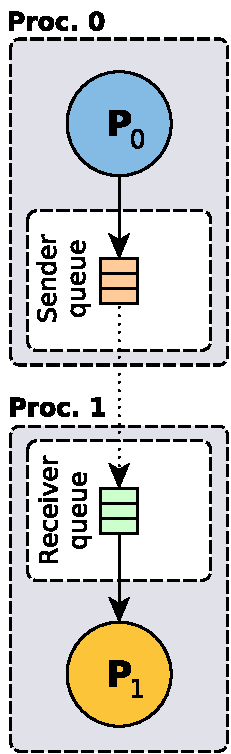
\includegraphics[width=0.3\linewidth]{figures/mpi-spsc-queue.pdf}
  \caption{Diagrama de colas SPSC.}
  %\label{fig:sub1}
\end{subfigure}%
\hfill
\begin{subfigure}[b]{.5\textwidth}
  \centering
  \includegraphics[width=0.5\linewidth]{figures/mpi-spsc-communication.pdf}
  \caption{Protocolo de comunicación de colas SPSC.}
  %\label{fig:sub2}
\end{subfigure}
\caption{Diagrama y protocolo de comunicación de colas SPSC.}
\label{fig:spsc-queue}
\end{figure}
\vspace{0.35cm}

El lado izquierdo de las Figuras ~\ref{fig:spsc-queue} y~\ref{fig:mpmc-queue} muestran, respectivamente, los diagramas de cola en los escenarios de SPSC y MPMC.\footnote{Consideramos el SPMC y MPSC los escenarios se implementan utilizando el modo de cola MPMC, ya que estos casos se pueden ver como especializaciones de MPMC.} Como se muestra en el lado del productor de colas MPMC, la cola crea un subproceso de controlador por proceso de productor ($T$) para solapar las comunicaciones con los cálculos del operador. La cola también selecciona un hilo del controlador que actúa como el orquestador, que es responsable de gestionar la cola haciendo un seguimiento de los artículos disponibles en cada productor y reenviando las solicitudes de artículos de consumo a un productor determinado. Sin embargo, para la cola de SPSC, dado que los procesos de productor y consumidor son conocidos de antemano, las comunicaciones pueden superponerse con cálculos utilizando directamente primitivas de envío/recepción asíncronas de \acrshort{mpi}. Por lo tanto, no se necesitan subprocesos de controlador en el lado del productor para administrar la cola cuando se trata de escenarios de SPSC.

Para implementar el comportamiento mencionado anteriormente, los lados de cola de \acrshort{mpi} del productor y del consumidor se comunican siguiendo un protocolo específico dependiendo del modo de cola ((ver lado derecho de las Figuras~\ref{fig:spsc-queue} y~\ref{fig:mpmc-queue} para SPSC y MPMC, respectivamente). Este protocolo de comunicación se compone de las tres fases siguientes:

\begin{itemize}
\item \textbf{Fase de configuración}: el objetivo de esta fase es determinar si la cola debe ejecutarse en modo SPSC o MPMC. Si solo hay un productor y un consumidor, entonces la cola se configura como SPSC; de lo contrario, se establece como MPMC. Al comienzo de esta fase, tanto productores como consumidores inicializan sus lados de cola de acuerdo con el tipo de operador (etapa de Pipeline o réplica de Farm). A partir de este momento, todos los procesos intercambian diferentes mensajes de configuración con el proceso del orquestador para seleccionar el modo de cola. Primero, los consumidores y productores respectivamente envían los mensajes \texttt{reg\_recv<id, type>} y \texttt{reg\_send<id>} para registrarse en el orquestador. Además, los consumidores indican el orquestador su \texttt{type}, es decir, la etapa de Pipeline o la réplica de Farm. A continuación, el orquestador configura la cola como SPSC o MPMC según la cantidad de consumidores y productores registrados, y les comunica el modo de cola final (\texttt{ack<mode>}). Finalmente, los procesos de los productores inician los hilos de controlador correspondientes si la cola está configurada como MPMC.

\item \textbf{Fase de comunicación}: se usa un protocolo de comunicación diferente dependiendo del modo de cola. Si la cola está configurada como SPSC, el proceso del productor envía los artículos de manera asíncrona al consumidor. De lo contrario, si la cola está configurada en modo MPMC, el hilo del orquestador espera mensajes provenientes de productores y consumidores. Los productores envían mensajes \texttt{notify\_item<id>} para informar sobre un nuevo artículo disponible, mientras que los consumidores envían \texttt{item\_req<id>} para pedirle al orquestador un artículo. Cuando el orquestador recibe una nueva solicitud, sirve el artículo directamente o reenvía la solicitud a otro productor, siguiendo el mismo orden en el que llegaron las notificaciones del productor.

\vspace{0.35cm}
\begin{figure}[!tbp]
\centering
\begin{subfigure}[b]{0.5\textwidth}
  \centering
  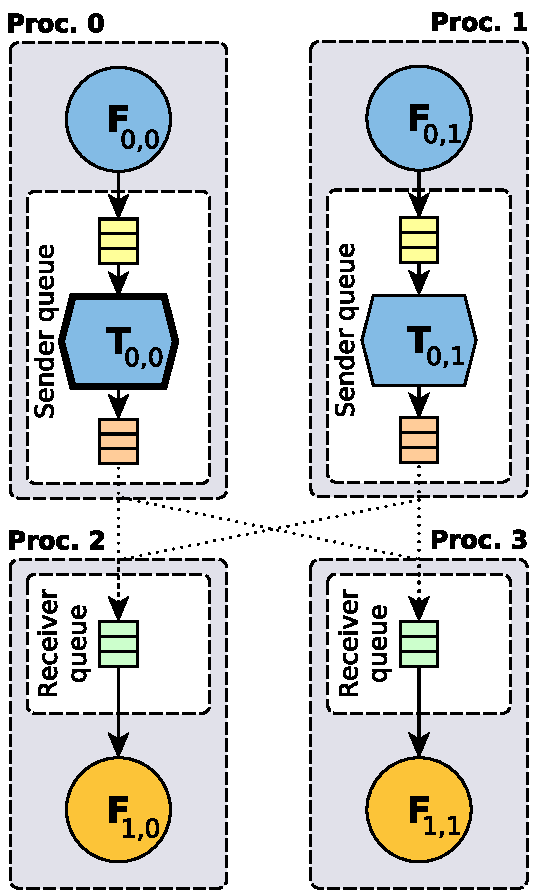
\includegraphics[width=0.55\linewidth]{figures/mpi-mpmc-queue.pdf}
  \caption{Diagrama de colas MPMC.}
  \label{fig:sub1}
\end{subfigure}%
\hfill
\begin{subfigure}[b]{0.5\textwidth}
  \centering
  \includegraphics[width=0.95\linewidth]{figures/mpi-mpmc-communication.pdf}
  \caption{Protocolo de comunicación de colas MPMC.}
  \label{fig:sub2}
\end{subfigure}
\caption{Diagrama y protocolo de comunicación de colas MPMC.}
\label{fig:mpmc-queue}
\end{figure}
\vspace{0.35cm}

\item \textbf{Fase de finalización}: Similar a la fase anterior, se usa un protocolo de terminal diferente dependiendo del modo de cola. Para el modo SPSC, tan pronto como el productor finaliza su operación, envía el mensaje \emph{end-of-stream} (\texttt{EOS}) al consumidor. Por el contrario, para el modo MPMC, el orquestador espera mensajes de \texttt{EOS} de todos los productores, incluido su propio elemento de terminación. Cuando esto sucede, el orquestador envía a cada uno de los consumidores el mensaje \texttt{EOS} para finalizar la comunicación.
\end{itemize}

Gracias a estas colas, los operadores de stream ejecutados por procesos \acrshort{mpi} pueden transmitir elementos de acuerdo con el flujo de stream dictado por una construcción de Pipeline concreta, que puede estar compuesta por diferentes patrones de Farm. Tenga en cuenta que si un proceso utiliza varias instancias de cola simultáneamente, las etiquetas \acrshort{mpi}, en lugar de múltiples comunicadores, se utilizan para hacer referencia a cada una de ellas.

\subsection{Algoritmo de distribución de operadores en procesos \acrshort{mpi}}
\label{sec:algoritmo_distribucion_mpi}

La política de ejecución de \acrshort{mpi} también incorpora un algoritmo de asignación para asignar operadores de flujo en procesos \acrshort{mpi}. Básicamente, este algoritmo calcula al comienzo de la ejecución de la tubería la cantidad total de operadores involucrados en ella, considerando tanto el número de etapas como las réplicas de la granja. Luego, calcula la cantidad de operadores que se deben ejecutar por proceso de \acrshort{mpi} ($opp$). Por defecto, los operadores se distribuyen homogéneamente usando la fórmula:

\vspace{0.35cm}
\begin{equation}\label{eq:opp}
opp= \frac{num\_ops}{num\_procs}
\end{equation}
\vspace{0.35cm}

Sin embargo, el usuario puede anular este valor llamando a la función \texttt{set\_grouping\_granularity(int ops\_per\_proc)}, parte de la clase de política de ejecución de \acrshort{mpi}. A continuación, cada uno de los procesos de \acrshort{mpi} calcula, utilizando su rango, el rango de operadores que deberían ejecutarse con la siguiente fórmula:

\vspace{0.35cm}
\begin{gather}\label{eq:range}
  Range(rank) =
  \begin{cases}
  \{rank * opp, ((rank+1)*opp)-1\} & \text{if $rank\neq num\_procs-1$} \\
  \{rank * opp, num\_ops-1\} & \text{if $rank=num\_procs-1$} 
  \end{cases}
\end{gather}

\vspace{0.35cm}
\begin{figure*}[ht!]
  \centering
  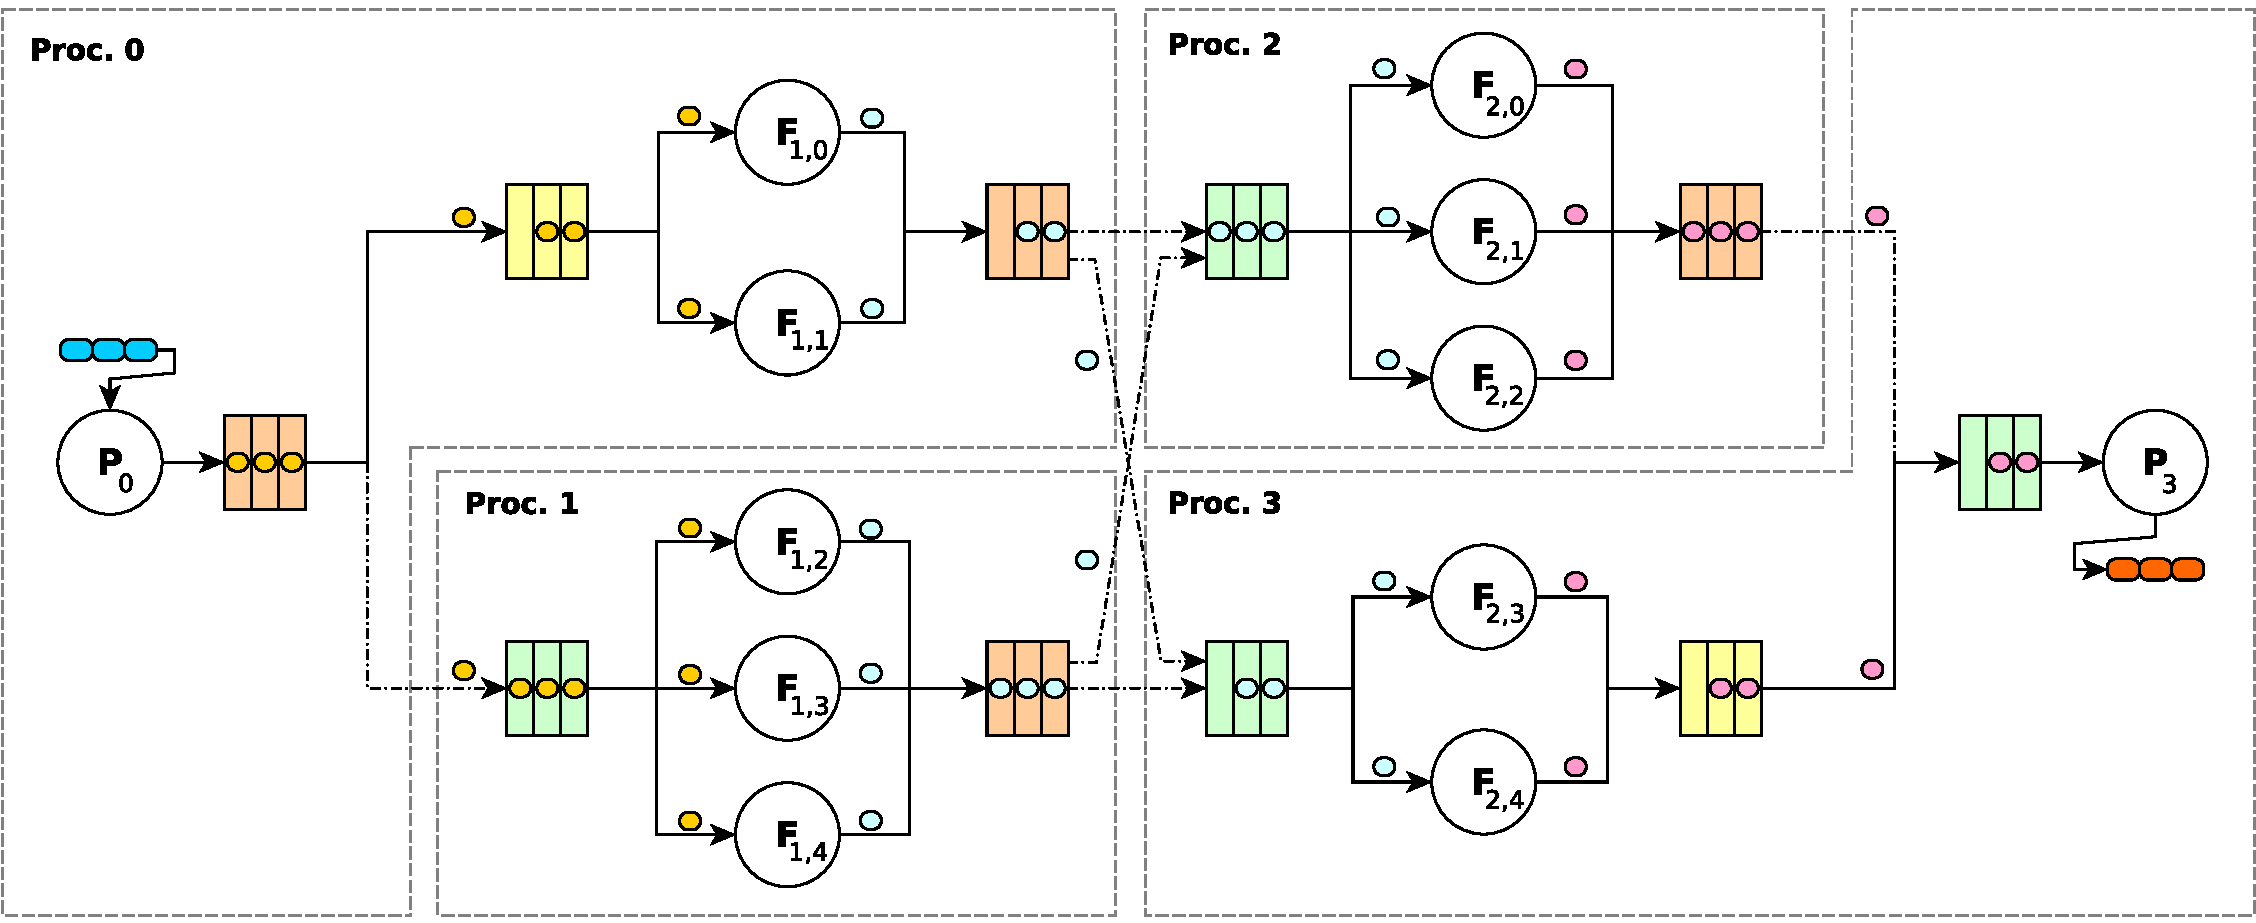
\includegraphics[width=0.95\textwidth]{figures/pipeline-mapping.pdf}\vspace{-0.2cm}
  \caption{Distribución de operadores de stream en procesos con $opp=3$.}\label{fig:mapping}
\end{figure*}
\vspace{0.35cm}

De acuerdo con esta fórmula, si el valor de $opp$ se establece de manera predeterminada, es decir, con Ec.~\ref{eq:opp}, todos los procesos ejecutan el mismo número de operadores excepto el último, que ejecuta todos los operadores restantes. De lo contrario, si $opp$ ha sido establecido por el usuario y es mayor que el establecido por defecto, entonces algunos últimos procesos podrían no ejecutar ningún operador. Tenga en cuenta también que el algoritmo de distribución selecciona operadores consecutivos para mapearlos en procesos \acrshort{mpi}, es decir, siguiendo el mismo orden en el que aparecen en el patrón de Pipeline.

La Figura~\ref{fig:mapping} representa una tubería de cuatro etapas compuesta por dos patrones de granja en la segunda y tercera etapas, que se ejecuta con 5 réplicas cada una. En este caso, la granularidad de agrupación o $opp$ se ha calculado de forma predeterminada utilizando Ec.~\ref{eq:opp}. Dado que cada proceso ejecuta los 3 operadores consecutivos correspondientes a los devueltos por Ec.~\ref{eq:range}. Por lo tanto, el mismo proceso de \acrshort{mpi} puede ejecutarse, utilizando la política de memoria compartida local, en etapas de Pipeline y/o réplicas de Farm. 

En general, esta política de ejecución de \acrshort{mpi} permite que los patrones \acrshort{grppi} se ejecuten en plataformas distribuidas de múltiples núcleos, aprovechando el paralelismo inter e intranodo. Además, gracias a su algoritmo de distribución de operadores, es capaz de distribuir automáticamente operadores siguiendo el orden lógico de transmisión.

%This policy allows the hybrid execution of those patterns when the number of total operators (\Pipeline stages and \Farm replicas) is higher than the number of \acrshort{mpi} processes. This is accomplished by collapsing contiguous \Pipeline operators or \Farm replicas onto multi-threaded processes.

% \begin{lstlisting}[linewidth=1\columnwidth,caption={SPSC queue of the \acrshort{mpi} back end.},label={lst:mpi-spsc-queue},frame=single]
% #include <boost/mpi.hpp>
% template <typename T>
% class mpi_spsc_queue {
%  private:
%   std::deque<mpi::request> buffer_;
%   int buffer_size_, rank_recv_;
%   bool pending_req_= false;
%   mpi::request req;
%   T item_;
%   ...
%  public:
%   ...
%   bool push (T item) {
%     // check for done requests
%     while (!buffer_.empty()) {
%       auto req = buffer_.front();
%       req.test() ? buffer_.pop_front() : break;
%     }
%     // send item async and store request
%     buffer_.push_back(comm_.isend(rank_recv_, tag_, item));
%   };
%   T pop() {
%     // request for the first element
%     if (!pending_req_) {
%       req = comm_.irecv(mpi::any_source, tag_, item_);
%       pending_req_ = true;
%     }
%     // wait for the previous item and request the next one
%     req.wait();
%     T item = item_;
%     req = comm_.irecv(mpi::any_source, tag_, item_);
%     return item;
%   };
% } 
% \end{lstlisting}

%\afterpage{\blankpage} % blank page
